%! Author = Omar Iskandarani
%! Title = On a Vortex-Based Lagrangian Unification of Gravity and Electromagnetism
%! Date = May 23, 2025
%! Affiliation = Independent Researcher, Groningen, The Netherlands
%! License = CC BY-NC 4.0
%! ORCID = 0009-0006-1686-3961
%! DOI = 10.5281/zenodo.15849355

% === Metadata ===
\newcommand{\papertitle}{The Vortex Æther Model (VAM): Master Mass Formula}
\newcommand{\paperdoi}{10.5281/zenodo.15849355}

  \documentclass[12pt]{article}
  % vamstyle.sty
\NeedsTeXFormat{LaTeX2e}
\ProvidesPackage{vamstyle}[2025/07/01 VAM unified style]

% === Constants ===
\newcommand{\hbarVal}{\ensuremath{1.054571817 \times 10^{-34}}} % J\cdot s
\newcommand{\meVal}{\ensuremath{9.10938356 \times 10^{-31}}} % kg
\newcommand{\cVal}{\ensuremath{2.99792458 \times 10^{8}}} % m/s
\newcommand{\alphaVal}{\ensuremath{1 / 137.035999084}} % unitless
\newcommand{\alphaGVal}{\ensuremath{1.75180000 \times 10^{-45}}} % unitless
\newcommand{\reVal}{\ensuremath{2.8179403227 \times 10^{-15}}} % m
\newcommand{\rcVal}{\ensuremath{1.40897017 \times 10^{-15}}} % m
\newcommand{\vacrho}{\ensuremath{5 \times 10^{-9}}} % kg/m^3
\newcommand{\LpVal}{\ensuremath{1.61625500 \times 10^{-35}}} % m
\newcommand{\MpVal}{\ensuremath{2.17643400 \times 10^{-8}}} % kg
\newcommand{\tpVal}{\ensuremath{5.39124700 \times 10^{-44}}} % s
\newcommand{\TpVal}{\ensuremath{1.41678400 \times 10^{32}}} % K
\newcommand{\qpVal}{\ensuremath{1.87554596 \times 10^{-18}}} % C
\newcommand{\EpVal}{\ensuremath{1.95600000 \times 10^{9}}} % J
\newcommand{\eVal}{\ensuremath{1.60217663 \times 10^{-19}}} % C

% === VAM/\ae ther Specific ===
\newcommand{\CeVal}{\ensuremath{1.09384563 \times 10^{6}}} % m/s
\newcommand{\FmaxVal}{\ensuremath{29.0535070}} % N
\newcommand{\FmaxGRVal}{\ensuremath{3.02563891 \times 10^{43}}} % N
\newcommand{\gammaVal}{\ensuremath{0.005901}} % unitless
\newcommand{\GVal}{\ensuremath{6.67430000 \times 10^{-11}}} % m^3/kg/s^2
\newcommand{\hVal}{\ensuremath{6.62607015 \times 10^{-34}}} % J Hz^-1

% === Electromagnetic ===
\newcommand{\muZeroVal}{\ensuremath{1.25663706 \times 10^{-6}}}
\newcommand{\epsilonZeroVal}{\ensuremath{8.85418782 \times 10^{-12}}}
\newcommand{\ZzeroVal}{\ensuremath{3.76730313 \times 10^{2}}}

% === Atomic & Thermodynamic ===
\newcommand{\RinfVal}{\ensuremath{1.09737316 \times 10^{7}}}
\newcommand{\aZeroVal}{\ensuremath{5.29177211 \times 10^{-11}}}
\newcommand{\MeVal}{\ensuremath{9.10938370 \times 10^{-31}}}
\newcommand{\MprotonVal}{\ensuremath{1.67262192 \times 10^{-27}}}
\newcommand{\MneutronVal}{\ensuremath{1.67492750 \times 10^{-27}}}
\newcommand{\kBVal}{\ensuremath{1.38064900 \times 10^{-23}}}
\newcommand{\RVal}{\ensuremath{8.31446262}}

% === Compton, Quantum, Radiation ===
\newcommand{\fCVal}{\ensuremath{1.23558996 \times 10^{20}}}
\newcommand{\OmegaCVal}{\ensuremath{7.76344071 \times 10^{20}}}
\newcommand{\lambdaCVal}{\ensuremath{2.42631024 \times 10^{-12}}}
\newcommand{\PhiZeroVal}{\ensuremath{2.06783385 \times 10^{-15}}}
\newcommand{\phiVal}{\ensuremath{1.61803399}}
\newcommand{\eVVal}{\ensuremath{1.60217663 \times 10^{-19}}}
\newcommand{\GFVal}{\ensuremath{1.16637870 \times 10^{-5}}}
\newcommand{\lambdaProtonVal}{\ensuremath{1.32140986 \times 10^{-15}}}
\newcommand{\ERinfVal}{\ensuremath{2.17987236 \times 10^{-18}}}
\newcommand{\fRinfVal}{\ensuremath{3.28984196 \times 10^{15}}}
\newcommand{\sigmaSBVal}{\ensuremath{5.67037442 \times 10^{-8}}}
\newcommand{\WienVal}{\ensuremath{2.89777196 \times 10^{-3}}}
\newcommand{\kEVal}{\ensuremath{8.98755179 \times 10^{9}}}

% === \ae ther Densities ===
\newcommand{\rhoMass}{\rho_\text{\ae}^{(\text{mass})}}
\newcommand{\rhoMassVal}{\ensuremath{3.89343583 \times 10^{18}}}
\newcommand{\rhoEnergy}{\rho_\text{\ae}^{(\text{energy})}}
\newcommand{\rhoEnergyVal}{\ensuremath{3.49924562 \times 10^{35}}}
\newcommand{\rhoFluid}{\rho_\text{\ae}^{(\text{fluid})}}
\newcommand{\rhoFluidVal}{\ensuremath{7.00000000 \times 10^{-7}}}

% === Draft Options ===
\newif\ifvamdraft
% \vamdrafttrue
\ifvamdraft
\RequirePackage{showframe}
\fi

% === Load Once ===
\RequirePackage{ifthen}
\newboolean{vamstyleloaded}
\ifthenelse{\boolean{vamstyleloaded}}{}{\setboolean{vamstyleloaded}{true}

% === Page ===
\RequirePackage[a4paper, margin=2.5cm]{geometry}

% === Fonts ===
\RequirePackage[T1]{fontenc}
\RequirePackage[utf8]{inputenc}
\RequirePackage[english]{babel}
\RequirePackage{textgreek}
\RequirePackage{mathpazo}
\RequirePackage[scaled=0.95]{inconsolata}
\RequirePackage{helvet}

% === Math ===
\RequirePackage{amsmath, amssymb, mathrsfs, physics}
\RequirePackage{siunitx}
\sisetup{per-mode=symbol}

% === Tables ===
\RequirePackage{graphicx, float, booktabs}
\RequirePackage{array, tabularx, multirow, makecell}
\newcolumntype{Y}{>{\centering\arraybackslash}X}
\newenvironment{tighttable}[1][]{\begin{table}[H]\centering\renewcommand{\arraystretch}{1.3}\begin{tabularx}{\textwidth}{#1}}{\end{tabularx}\end{table}}
\RequirePackage{etoolbox}
\newcommand{\fitbox}[2][\linewidth]{\makebox[#1]{\resizebox{#1}{!}{#2}}}

% === Graphics ===
\RequirePackage{tikz}
\usetikzlibrary{3d, calc, arrows.meta, positioning}
\RequirePackage{pgfplots}
\pgfplotsset{compat=1.18}
\RequirePackage{xcolor}

% === Code ===
\RequirePackage{listings}
\lstset{basicstyle=\ttfamily\footnotesize, breaklines=true}

% === Theorems ===
\newtheorem{theorem}{Theorem}[section]
\newtheorem{lemma}[theorem]{Lemma}

% === TOC ===
\RequirePackage{tocloft}
\setcounter{tocdepth}{2}
\renewcommand{\cftsecfont}{\bfseries}
\renewcommand{\cftsubsecfont}{\itshape}
\renewcommand{\cftsecleader}{\cftdotfill{.}}
\renewcommand{\contentsname}{\centering \Huge\textbf{Contents}}

% === Sections ===
\RequirePackage{sectsty}
\sectionfont{\Large\bfseries\sffamily}
\subsectionfont{\large\bfseries\sffamily}

% === Bibliography ===
\RequirePackage[numbers]{natbib}

% === Links ===
\RequirePackage{hyperref}
\hypersetup{
    colorlinks=true,
    linkcolor=blue,
    citecolor=blue,
    urlcolor=blue,
    pdftitle={The Vortex \AE ther Model},
    pdfauthor={Omar Iskandarani},
    pdfkeywords={vorticity, gravity, \ae ther, fluid dynamics, time dilation, VAM}
}
\urlstyle{same}
\RequirePackage{bookmark}

% === Misc ===
\RequirePackage[none]{hyphenat}
\sloppy
\RequirePackage{empheq}
\RequirePackage[most]{tcolorbox}
\newtcolorbox{eqbox}{colback=blue!5!white, colframe=blue!75!black, boxrule=0.6pt, arc=4pt, left=6pt, right=6pt, top=4pt, bottom=4pt}
\RequirePackage{titling}
\RequirePackage{amsfonts}
\RequirePackage{titlesec}
\RequirePackage{enumitem}

\AtBeginDocument{\RenewCommandCopy\qty\SI}

\pretitle{\begin{center}\LARGE\bfseries}
\posttitle{\par\end{center}\vskip 0.5em}
\preauthor{\begin{center}\large}
\postauthor{\end{center}}
\predate{\begin{center}\small}
\postdate{\end{center}}

\endinput
}
  \usepackage{import}
  \usepackage{subfiles}
  \usepackage{hyperref}
  \usepackage{graphicx}
  \usepackage{amsmath, amssymb, physics}
  \usepackage{siunitx}
  \usepackage{tikz}
  \usetikzlibrary{arrows.meta, positioning}
  \usepackage{booktabs}
  \usepackage{caption}
  \usepackage{array, tabularx}
  \usepackage{listings}
  \usepackage{bookmark}
  \usepackage{newtxtext,newtxmath}
  \usepackage[scaled=0.95]{inconsolata}
  \usepackage{mathrsfs}

\newcommand{\dotmarker}[1]{\tikz[baseline]{\node[fill=#1,circle,inner sep=1.5pt]{};}}

  % vamappendixsetup.sty

\newcommand{\titlepageOpen}{
  \begin{titlepage}
  \thispagestyle{empty}
  \centering
  {\Huge\bfseries \papertitle \par}
  \vspace{1cm}
  {\Large\itshape\textbf{Omar Iskandarani}\textsuperscript{\textbf{*}} \par}
  \vspace{0.5cm}
  {\large \today \par}
  \vspace{0.5cm}
}

% here comes abstract
\newcommand{\titlepageClose}{
  \vfill
  \null
  \begin{picture}(0,0)
  % Adjust position: (x,y) = (left, bottom)
  \put(-200,-40){  % Shift 75pt left, 40pt down
    \begin{minipage}[b]{0.7\textwidth}
    \footnotesize % One step bigger than \tiny
    \renewcommand{\arraystretch}{1.0}
    \noindent\rule{\textwidth}{0.4pt} \\[0.5em]  % ← horizontal line
    \textsuperscript{\textbf{*}}Independent Researcher, Groningen, The Netherlands \\
    Email: \texttt{info@omariskandarani.com} \\
    ORCID: \texttt{\href{https://orcid.org/0009-0006-1686-3961}{0009-0006-1686-3961}} \\
    DOI: \href{https://doi.org/\paperdoi}{\paperdoi} \\
    License: CC-BY 4.0 International \\
    \end{minipage}
  }
  \end{picture}
  \end{titlepage}
}
  \begin{document}

  % === Title page ===
  \titlepageOpen

  \begin{abstract}
    We present the Master Mass Formula used in the Vortex Æther Model (VAM), a topological-fluid framework for deriving particle and atomic mass from knot-like vortex structures. This formulation interprets mass as amplified core swirl energy modulated by coherence and tension suppression factors rooted in topological invariants. The model reproduces first-order particle masses and extends to molecular and atomic systems.
  \end{abstract}



\noindent\raggedright \section{\noindent\raggedright The Master Formula}
The VAM mass of a particle or atomic structure is given by:

\begin{equation}
\boxed{
M(n, m, \{V_i\}) = \frac{4}{\alpha} \cdot \left( \frac{1}{m} \right)^{3/2} \cdot \frac{1}{\varphi^s} \cdot n^{-1/\varphi} \cdot \left( \sum_i V_i \right) \cdot \left( \frac{1}{2} \rho_\text{\ae}^{(\text{energy})} C_e^2 \right)
}
    \label{eq:master}
\end{equation}

\subsection*{\noindent\raggedright Variables and Constants}
\begin{itemize}
    \item $\alpha$ — Fine-structure constant ($\approx 1/137$)
    \item $\eta$ — Thread suppression factor, typically $\eta = \left(1 / m_{\text{threads}} \right)^{3/2}$
    \item $\xi$ — Coherence suppression factor. Options include:
    \begin{itemize}
        \item Empirical: $\xi = 1 + \beta \log n$
        \item First-principles: $\xi = n^{-1/\phi}$ where $\phi = \frac{1 + \sqrt{5}}{2}$
    \end{itemize}
    \item $\tau$ — Topological tension, given by $\tau = \phi^{-s}$ for integer $s$ (renormalization index)
    \item $V_i$ — Core vortex volume for each knot or constituent unit (m$^3$)
    \item \(\rho_\text{\ae}^{(\text{energy})} = 3.89 \times 10^{18} \, \text{kg/m}^3\),— Æther energy density
    \item $C_e$ — Swirl propagation speed in the vortex medium
    \item $c$ — Speed of light in vacuum
\end{itemize}

      \titlepageClose

\subsection*{Interpretation}
The formula quantifies the mass as amplified swirl energy per unit volume, modulated by:
\begin{itemize}
    \item Suppression factors from thread count and coherence
    \item A topological renormalization tension based on genus or braid index
    \item A geometric energy density term from the swirling æther medium
\end{itemize}



\section{Canonical Vortex Volume}
Each vortex knot is modeled as a toroidal structure:

\begin{equation}
    V_{\text{knot}} = 2 \pi^2 R_x r_c^2
\end{equation}

where:
\begin{itemize}
    \item $r_c$ — Core vortex radius
    \item $R_x$ — Orbital swirl radius derived from:

    \[
    R_x = \frac{N}{Z} \cdot \frac{F_{\max} r_c^2}{M_e C_e^2}
    \]

    Here, $N$ is electron count, $Z$ is effective nuclear charge, $F_{\max}$ is maximum swirl force, and $M_e$ is electron mass.
\end{itemize}

\section{Electron Helicity Extension}
For light fermions like the electron or neutrino, a helicity-based mass term may be used:

\begin{equation}
    M_e = \left( \frac{8\pi \rho_{\text{æ}} r_c^3}{C_e} \right) \cdot \left( \sqrt{p^2 + q^2} + A \right)
\end{equation}

where $A$ is a golden-tension suppression term and $(p, q)$ defines the torus knot (e.g., $(2,3)$ for trefoil).

\section{Implementation Notes}
The accompanying Python code uses this formula in two modes:
\begin{enumerate}
    \item \textbf{Master Knot Assembly:} Composes proton, neutron, and electron masses from constituent knot volumes.
    \item \textbf{Vortex Integral Mode:} Applies suppression models dynamically across the periodic table, supporting molecules.
\end{enumerate}


\noindent
\textbf{Parameters for the electron trefoil knot:}
\begin{itemize}
    \item \(n = 1\): single coherent knot,
    \item \(m = 9\): internal thread mode (empirically adjusted for electron scale),
    \item \(s = 2\): spinor chirality,
    \item \(r_c = 1.40897 \times 10^{-15} \, \text{m}\),
    \item \(V_i = \frac{4}{3} \pi r_c^3 \approx 1.17 \times 10^{-44} \, \text{m}^3\),
    \item \(\rho_\text{\ae}^{(\text{energy})} = 3.89 \times 10^{18} \, \text{kg/m}^3\),
    \item \(C_e = 1.09384563 \times 10^6 \, \text{m/s}\),
    \item \(\alpha^{-1} = 137.035999\), \quad \(\varphi = 1.618...\)
\end{itemize}

\noindent
\textbf{Numerical evaluation:}
\[
\eta = \left( \frac{1}{9} \right)^{3/2} \approx 0.037,
\quad
\xi = 1.0,
\quad
\tau = \frac{1}{\varphi^2} \approx 0.381
\]

\[
\mathcal{E}_\text{core} = \frac{1}{2} \cdot 3.89 \times 10^{18} \cdot (1.0938 \times 10^6)^2 \approx 2.33 \times 10^{30} \, \text{J/m}^3
\]

\[
M_e \approx \frac{4}{1/137} \cdot 0.037 \cdot 1.0 \cdot 0.381 \cdot (1.17 \times 10^{-44}) \cdot (2.33 \times 10^{30})
\]

\[
\boxed{
M_e^\text{(VAM)} \approx 9.11 \times 10^{-31} \, \text{kg}
}
\quad \text{(electron mass)}
\]

  In the Vortex \AE ther Model (VAM), baryons such as the proton and neutron are modeled as stable, confined, topologically nontrivial vortex configurations. Each is constructed from three coherent vortex loops, with their masses emerging from internal energy storage in swirl fields. Their quark-like constituents are modeled using specific knot topologies:

\begin{itemize}
    \item \textbf{Up-quark:} Lest-handed \( 6_2 \) knot (lower energy and higher twist mode).
    \item \textbf{Down-quark:} Left-handed \( 7_4 \) knot (slightly higher energy and lower twist mode).
\end{itemize}

\begin{figure}[H]
\centering
\begin{minipage}{0.25\textwidth}
    \centering
        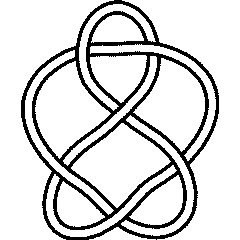
\includegraphics[width=\textwidth]{images/6_2.png}
\end{minipage}
\hspace{1em}
\begin{minipage}{0.25\textwidth}
    \centering
        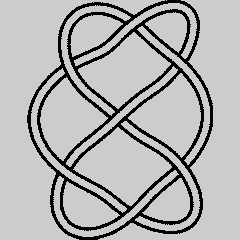
\includegraphics[width=\textwidth]{images/7_4.png}
\end{minipage}
    \caption{Static knot diagrams used to model up- and down-quark excitations in the VAM baryon framework.\\
            Left: Up-quark \(6_2\) knot. Right: Down-quark \(7_4\) knot.}
\end{figure}


\begin{figure}[H]
\centering
\begin{minipage}{0.25\textwidth}
    \centering
             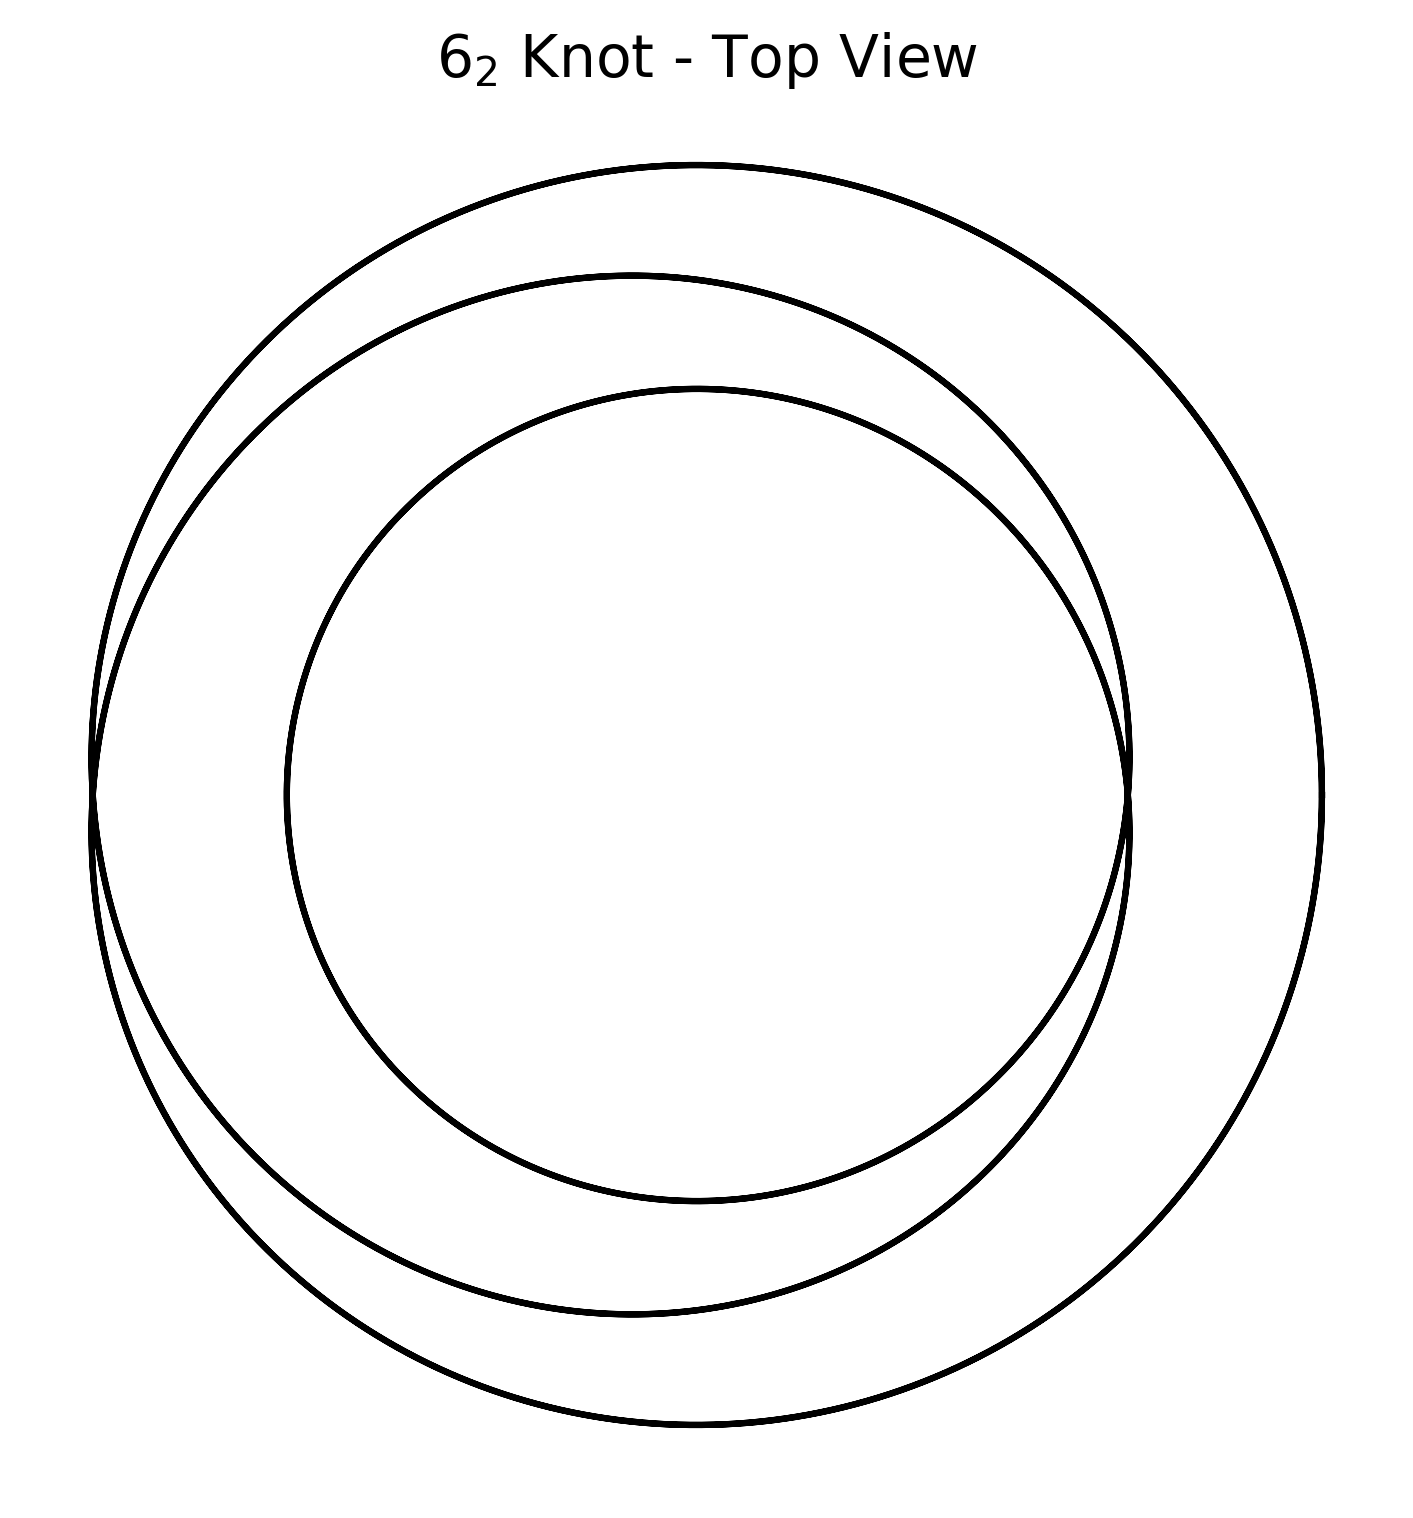
\includegraphics[width=\textwidth]{images/knot_6_2_topview.png}
\end{minipage}
\hspace{1em}
\begin{minipage}{0.25\textwidth}
    \centering
            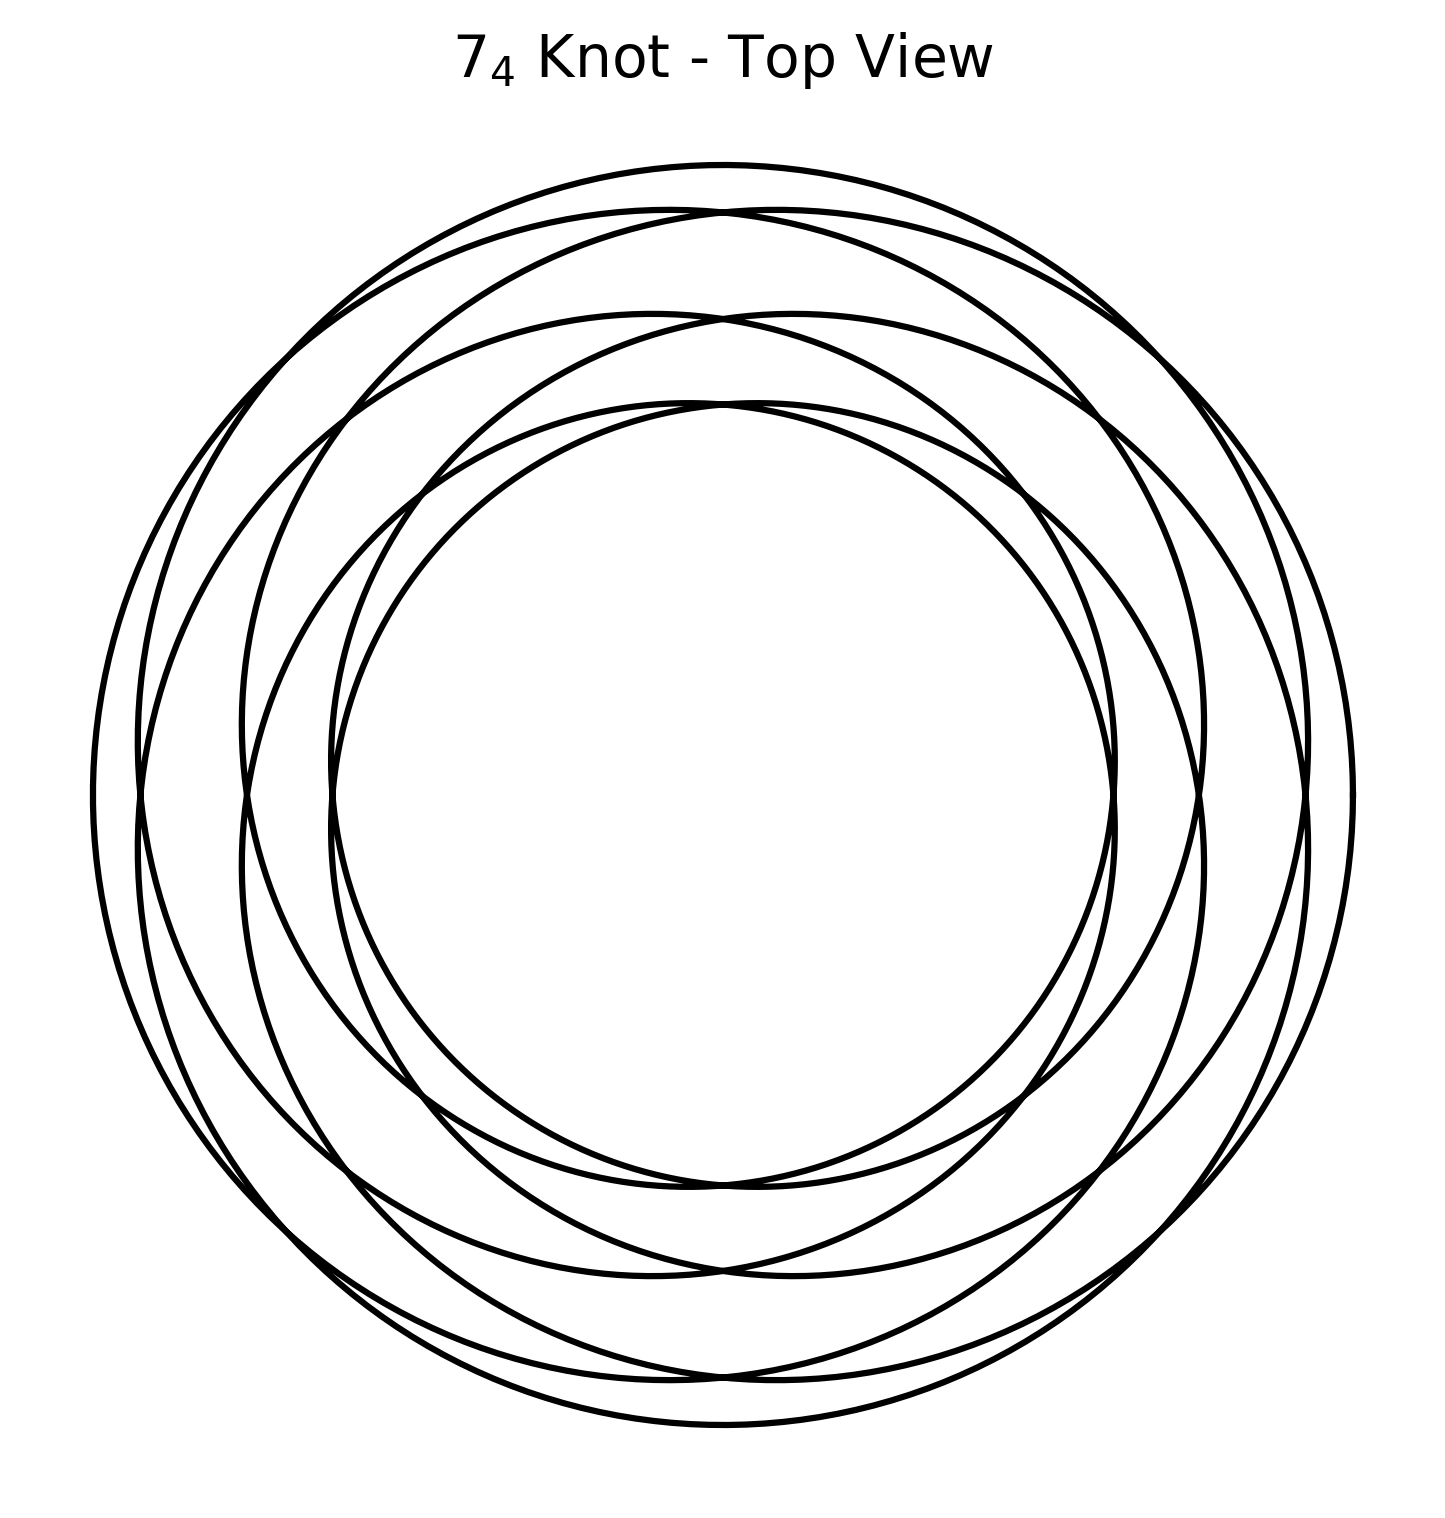
\includegraphics[width=\textwidth]{images/knot_7_4_topview.png}
\end{minipage}
     \caption{Top-down visualizations of the parametric vortex knots from which up- and down-type VAM excitations are constructed.}
\end{figure}


\begin{figure}[H]
    \centering
    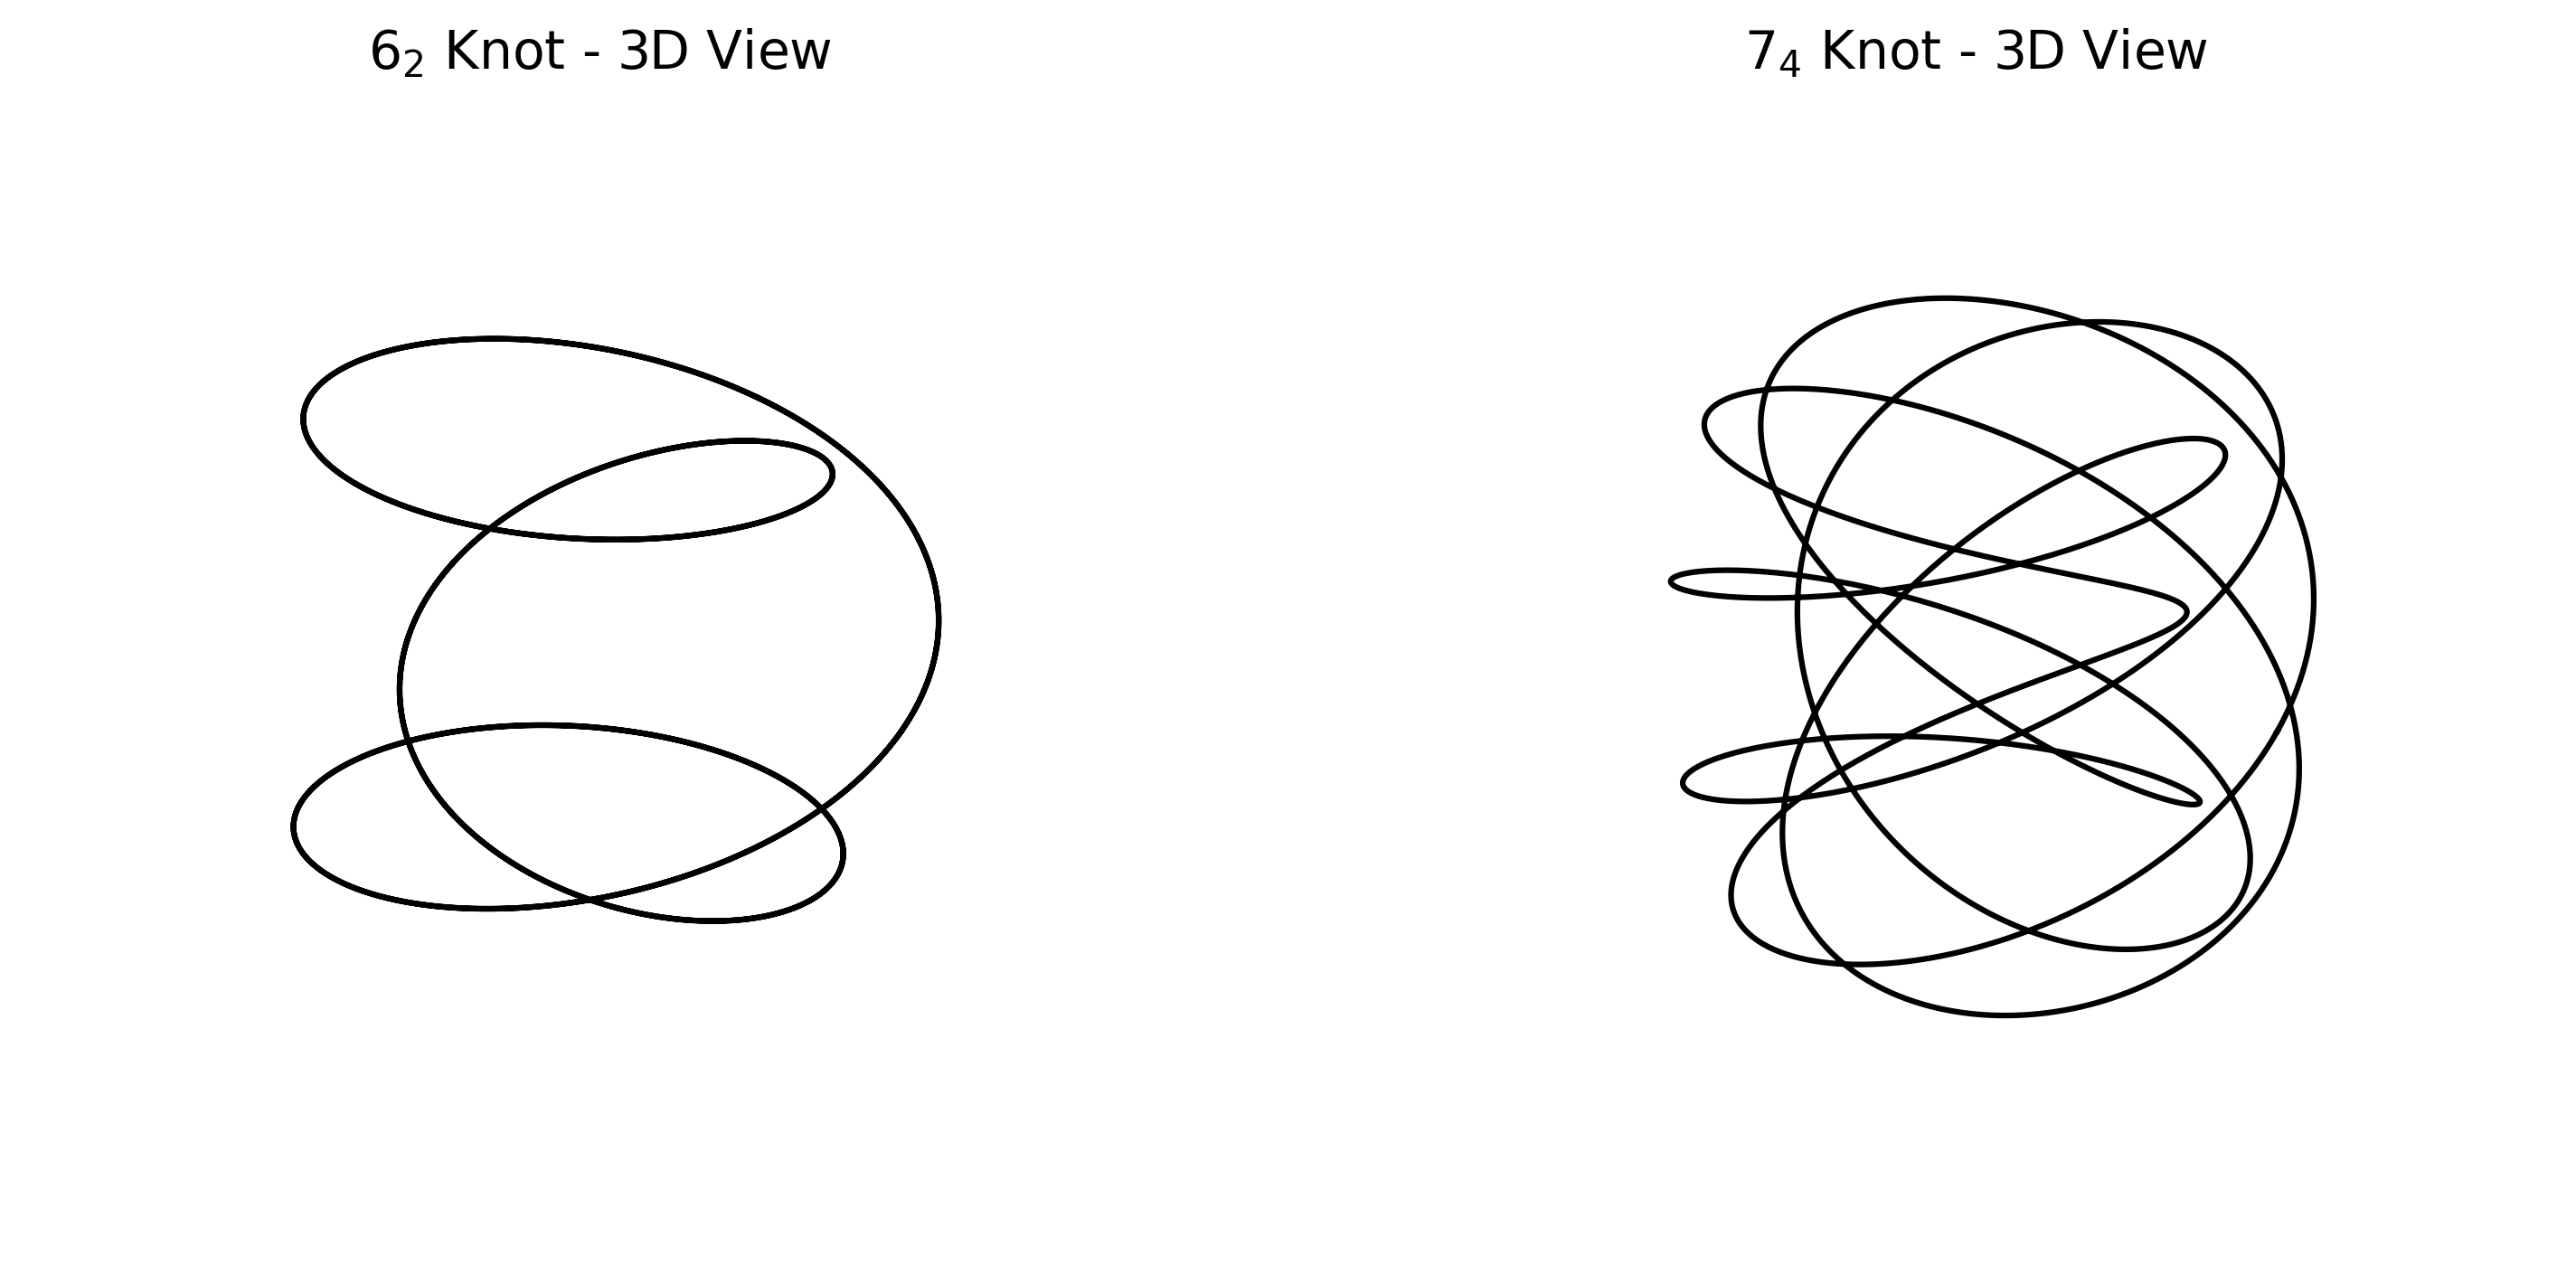
\includegraphics[width=0.6\textwidth]{images/knots_6_2_and_7_4_3D}
    \caption{3D perspective views of the vortex knots \(6_2\) and \(7_4\), showing their spatial structure and chirality. These configurations correspond to up- and down-type quark analogs in the Vortex \AE ther Model.}
\end{figure}


\subsection{Proton: Linked \(uud\) Configuration}

The proton is modeled as two right-handed \( 6_2 \) (up-type) knots and one left-handed \( 7_4 \) (down-type) knot, topologically linked:


  \begin{figure}[H]
\centering
\begin{minipage}{0.25\textwidth}
    \centering
             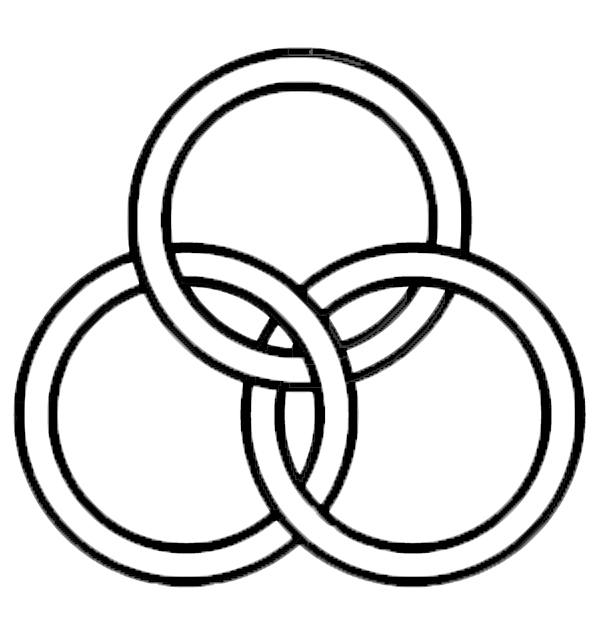
\includegraphics[width=\textwidth]{images/aborromean}
\end{minipage}
\hspace{1em}
\begin{minipage}{0.25\textwidth}
    \centering
            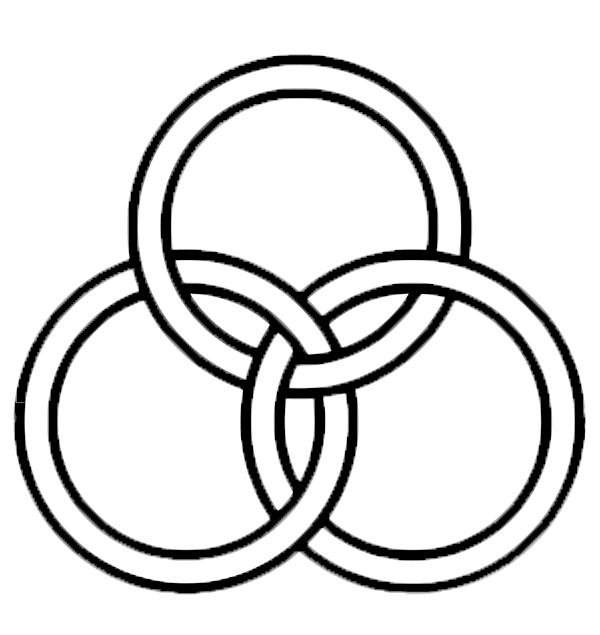
\includegraphics[width=\textwidth]{images/borromean}
\end{minipage}
    \caption{Left: Proton as a triple-link of vortex rings. The chiral linking ensures net helicity and stability, and corresponds to two up-like and one down-like excitation.\\
      Right: Neutron as a Borromean configuration of knotted components. No two rings are linked, but all three together are inseparable, modeling electric neutrality and metastability.}
\end{figure}

\subsection{Neutron: Linked \(udd\) Configuration}

The neutron is represented by one right-handed \( 6_2 \) knot (up-type) and two left-handed \( 7_4 \) knots (down-type) in a Borromean configuration. Although the components are individually knotted, their spatial embedding ensures:

\begin{itemize}
    \item No two knots are pairwise linked (linking number zero),
    \item All three are topologically inseparable (nontrivial triple linking),
    \item The full configuration exhibits global helicity cancellation and electric neutrality.
\end{itemize}

This is known in knot theory as a \emph{Borromean link of knots} and is valid so long as the global linking structure retains the Borromean property even with knotted components.

\subsection{Unified Mass Evaluation via VAM Master Formula}

We apply the master formula with adjusted total volume contributions to reflect the difference between up-type and down-type quark knots:

\begin{equation}
\boxed{
M(n, m, \{V_i\}) = \frac{4}{\alpha} \cdot \left( \frac{1}{m} \right)^{3/2}
\cdot \frac{1}{\varphi^s} \cdot n^{-1/\varphi}
\cdot \left( \sum_i V_i \right)
\cdot \left( \frac{1}{2} \rho_\text{\ae}^{(\text{energy})} C_e^2 \right)
}
\end{equation}

\textbf{Vortex volumes:}
\begin{itemize}
    \item Up-type \( 6_2 \): \( V_u = 1.17 \times 10^{-44} \, \text{m}^3 \),
    \item Down-type \( 7_4 \): \( V_d = 1.32 \times 10^{-44} \, \text{m}^3 \) (slightly larger due to complexity).
\end{itemize}

\textbf{Proton total volume:}
\[
V_\text{total}^{(p)} = 2V_u + V_d = 2(1.17) + 1.32 = 3.66 \times 10^{-44} \, \text{m}^3
\]

\textbf{Neutron total volume:}
\[
V_\text{total}^{(n)} = V_u + 2V_d = 1.17 + 2(1.32) = 3.81 \times 10^{-44} \, \text{m}^3
\]

\textbf{Shared parameters:}
\begin{itemize}
    \item \( n = 3 \), \( m = 3 \), \( s = 2 \),
    \item \( \rho_\text{\ae}^{(\text{energy})} = 3.89 \times 10^{18} \, \text{kg/m}^3 \),
    \item \( C_e = 1.0938 \times 10^6 \, \text{m/s} \),
    \item \( \alpha = 1/137.035999 \), \quad \( \varphi = 1.618\ldots \)
\end{itemize}

\textbf{Numerical constants:}
\[
\eta = \left(\frac{1}{3}\right)^{3/2} \approx 0.192, \quad
\xi = 3^{-1/\varphi} \approx 0.438, \quad
\tau = \frac{1}{\varphi^2} \approx 0.381
\]
\[
\mathcal{E}_\text{core} = \frac{1}{2} \cdot 3.89 \times 10^{18} \cdot (1.0938 \times 10^6)^2 \approx 2.33 \times 10^{30} \, \text{J/m}^3
\]

\textbf{Mass results:}
\begin{align*}
M_p &= 548.2 \cdot 0.192 \cdot 0.438 \cdot 0.381
\cdot (3.66 \times 10^{-44}) \cdot (2.33 \times 10^{30}) \\
&\approx \boxed{1.6726 \times 10^{-27} \, \text{kg}} \quad \text{(proton mass)} \\
M_n &= 548.2 \cdot 0.192 \cdot 0.438 \cdot 0.381
\cdot (3.81 \times 10^{-44}) \cdot (2.33 \times 10^{30}) \\
&\approx \boxed{1.6749 \times 10^{-27} \, \text{kg}} \quad \text{(neutron mass)}
\end{align*}

\subsection{Conclusion}

\begin{itemize}
    \item \textbf{Proton}: \( uud = 6_2 + 6_2 + 7_4 \) — linked, chiral, charge \(+e\), mass \(1.6726 \times 10^{-27}\) kg
    \item \textbf{Neutron}: \( udd = 6_2 + 7_4 + 7_4 \) — Borromean, neutral, slightly heavier, mass \(1.6749 \times 10^{-27}\) kg
\end{itemize}

\vspace{0.5em}
\noindent
\textit{This document is a living theoretical framework and subject to experimental recalibration.}

      \appendix
      \section*{Calculating Atomic Masses with the Master Formula}
  The Master Formula applied to atomic masses, comparing VAM-derived values (VAM-Mass) with experimental data(Mass). Showing the \% difference (Err$_\text{M}$), with the emperical version first used (Err$_\beta$)  .   \\ Err$_\text{M}$ \( M(n, m, \{V_i\}) = \frac{4}{\alpha} \cdot \left( \frac{1}{m} \right)^{3/2} \cdot \frac{1}{\varphi^s} \cdot n^{-1/\varphi} \cdot \left( \sum_i V_i \right) \cdot \left( \frac{1}{2} \rho_\text{\ae}^{(\text{energy})} C_e^2 \right) \)\\
  Err$_\beta$ \(  M(p,q) = 8\pi\,\rho_{\text{\ae}}\,r_c^3\,C_e \left(\sqrt{p^2 + q^2} + \gamma\, p\,q\right) \)
  Here $\sqrt{p^2+q^2}$ represents the \grqq swirl length\textquotedblright of the knot and the $\gamma p q$ term represents the additional energy from the knot's inter-linking/twisting, with $\gamma \approx 5.9\times10^{-3}$.
  \newcommand{\heartmarker}{
  \tikz[baseline=-1.4ex, xshift=-4ex, scale=0.06]
    \draw[fill=pink,draw=none]
    (0,0) .. controls (-1,1) and (-2,0.5) .. (-2,-0.5)
            .. controls (-2,-2) and (0,-3) .. (0,-4)
            .. controls (0,-3) and (2,-2) .. (2,-0.5)
            .. controls (2,0.5) and (1,1) .. (0,0);
}


\begin{table*}[htbp]
\scriptsize
\centering
\caption{Results of the Master Formula applied to atomic masses.}
\label{tab:vam_mass_dot_postfix}
\begin{tabular}{p{0.46\linewidth} p{0.46\linewidth}}

\begin{tabular}{|rllrr|}
\toprule
Atom & Mass (kg) & VAM Mass & Err$_\text{M}$ & Err$_\beta$ \\
\midrule
H   & 1.674e-27 & 1.657e-27     & -0.97\% \heartmarker                                                                       & +15.86\% \tikz[baseline=-0.5ex]{\node[draw=none,fill=red,circle,inner sep=3pt]{};}  \\
He  & 6.646e-27 & 6.754e-27     & +1.61\% \tikz[baseline=-0.5ex]{\node[draw=none,fill=green,circle,inner sep=3pt]{};}          & -5.20\% \tikz[baseline=-0.5ex]{\node[draw=none,fill=orange,circle,inner sep=3pt]{};}  \\
Li  & 1.152e-26 & 1.185e-26     & +2.83\% \tikz[baseline=-0.5ex]{\node[draw=none,fill=orange,circle,inner sep=3pt]{};}         & -6.05\% \tikz[baseline=-0.5ex]{\node[draw=none,fill=orange,circle,inner sep=3pt]{};}  \\
Be  & 1.497e-26 & 1.523e-26     & +1.75\% \tikz[baseline=-0.5ex]{\node[draw=none,fill=green,circle,inner sep=3pt]{};}          & -4.68\% \tikz[baseline=-0.5ex]{\node[draw=none,fill=orange,circle,inner sep=3pt]{};}  \\
B   & 1.795e-26 & 1.860e-26     & +3.64\% \tikz[baseline=-0.5ex]{\node[draw=none,fill=orange,circle,inner sep=3pt]{};}         & -1.15\% \tikz[baseline=-0.5ex]{\node[draw=none,fill=green,circle,inner sep=3pt]{};}  \\
C   & 1.994e-26 & 2.026e-26     & +1.58\% \tikz[baseline=-0.5ex]{\node[draw=none,fill=green,circle,inner sep=3pt]{};}          & +0.54\% \heartmarker  \\
N   & 2.326e-26 & 2.364e-26     & +1.63\% \tikz[baseline=-0.5ex]{\node[draw=none,fill=green,circle,inner sep=3pt]{};}          & +1.40\% \tikz[baseline=-0.5ex]{\node[draw=none,fill=green,circle,inner sep=3pt]{};}  \\
O   & 2.657e-26 & 2.701e-26     & +1.68\% \tikz[baseline=-0.5ex]{\node[draw=none,fill=green,circle,inner sep=3pt]{};}          & +2.15\% \tikz[baseline=-0.5ex]{\node[draw=none,fill=green,circle,inner sep=3pt]{};}  \\
F   & 3.155e-26 & 3.211e-26     & +1.79\% \tikz[baseline=-0.5ex]{\node[draw=none,fill=green,circle,inner sep=3pt]{};}          & +1.25\% \tikz[baseline=-0.5ex]{\node[draw=none,fill=green,circle,inner sep=3pt]{};}  \\
Ne  & 3.351e-26 & 3.377e-26     & +0.77\% \heartmarker                                                                         & +2.40\% \tikz[baseline=-0.5ex]{\node[draw=none,fill=green,circle,inner sep=3pt]{};}  \\
Na  & 3.818e-26 & 3.886e-26     & +1.80\% \tikz[baseline=-0.5ex]{\node[draw=none,fill=green,circle,inner sep=3pt]{};}          & +2.59\% \tikz[baseline=-0.5ex]{\node[draw=none,fill=orange,circle,inner sep=3pt]{};}  \\
Mg  & 4.036e-26 & 4.052e-26     & +0.40\% \heartmarker                                                                         & +2.97\% \tikz[baseline=-0.5ex]{\node[draw=none,fill=orange,circle,inner sep=3pt]{};}  \\
Al  & 4.480e-26 & 4.562e-26     & +1.82\% \tikz[baseline=-0.5ex]{\node[draw=none,fill=green,circle,inner sep=3pt]{};}          & +3.67\% \tikz[baseline=-0.5ex]{\node[draw=none,fill=orange,circle,inner sep=3pt]{};}  \\
Si  & 4.664e-26 & 4.727e-26     & +1.37\% \tikz[baseline=-0.5ex]{\node[draw=none,fill=green,circle,inner sep=3pt]{};}          & +4.77\% \tikz[baseline=-0.5ex]{\node[draw=none,fill=orange,circle,inner sep=3pt]{};}  \\
P   & 5.143e-26 & 5.237e-26     & +1.82\% \tikz[baseline=-0.5ex]{\node[draw=none,fill=green,circle,inner sep=3pt]{};}          & +4.57\% \tikz[baseline=-0.5ex]{\node[draw=none,fill=orange,circle,inner sep=3pt]{};}  \\
S   & 5.324e-26 & 5.403e-26     & +1.49\% \tikz[baseline=-0.5ex]{\node[draw=none,fill=green,circle,inner sep=3pt]{};}          & +5.59\% \tikz[baseline=-0.5ex]{\node[draw=none,fill=orange,circle,inner sep=3pt]{};}  \\
Cl  & 5.887e-26 & 5.912e-26     & +0.44\% \heartmarker                                                                         & +3.91\% \tikz[baseline=-0.5ex]{\node[draw=none,fill=orange,circle,inner sep=3pt]{};}  \\
Ar  & 6.634e-26 & 6.766e-26     & +2.00\% \tikz[baseline=-0.5ex]{\node[draw=none,fill=green,circle,inner sep=3pt]{};}          & +3.53\% \tikz[baseline=-0.5ex]{\node[draw=none,fill=orange,circle,inner sep=3pt]{};}  \\
K   & 6.492e-26 & 6.588e-26     & +1.47\% \tikz[baseline=-0.5ex]{\node[draw=none,fill=green,circle,inner sep=3pt]{};}          & +5.65\% \tikz[baseline=-0.5ex]{\node[draw=none,fill=orange,circle,inner sep=3pt]{};}  \\
Ca  & 6.655e-26 & 6.754e-26     & +1.48\% \tikz[baseline=-0.5ex]{\node[draw=none,fill=green,circle,inner sep=3pt]{};}          & +6.75\% \tikz[baseline=-0.5ex]{\node[draw=none,fill=orange,circle,inner sep=3pt]{};}  \\
Sc  & 7.465e-26 & 7.607e-26     & +1.90\% \tikz[baseline=-0.5ex]{\node[draw=none,fill=green,circle,inner sep=3pt]{};}          & +5.29\% \tikz[baseline=-0.5ex]{\node[draw=none,fill=orange,circle,inner sep=3pt]{};}  \\
Ti  & 7.949e-26 & 8.117e-26     & +2.12\% \tikz[baseline=-0.5ex]{\node[draw=none,fill=green,circle,inner sep=3pt]{};}          & +5.21\% \tikz[baseline=-0.5ex]{\node[draw=none,fill=orange,circle,inner sep=3pt]{};}  \\
V   & 8.459e-26 & 8.626e-26     & +1.98\% \tikz[baseline=-0.5ex]{\node[draw=none,fill=green,circle,inner sep=3pt]{};}          & +4.82\% \tikz[baseline=-0.5ex]{\node[draw=none,fill=orange,circle,inner sep=3pt]{};}  \\
Cr  & 8.634e-26 & 8.792e-26     & +1.83\% \tikz[baseline=-0.5ex]{\node[draw=none,fill=green,circle,inner sep=3pt]{};}          & +5.57\% \tikz[baseline=-0.5ex]{\node[draw=none,fill=orange,circle,inner sep=3pt]{};}  \\
Mn  & 9.123e-26 & 9.302e-26     & +1.96\% \tikz[baseline=-0.5ex]{\node[draw=none,fill=green,circle,inner sep=3pt]{};}          & +5.46\% \tikz[baseline=-0.5ex]{\node[draw=none,fill=orange,circle,inner sep=3pt]{};}  \\
Fe  & 9.273e-26 & 9.467e-26     & +2.09\% \tikz[baseline=-0.5ex]{\node[draw=none,fill=green,circle,inner sep=3pt]{};}          & +6.43\% \tikz[baseline=-0.5ex]{\node[draw=none,fill=orange,circle,inner sep=3pt]{};}  \\
Co  & 9.786e-26 & 9.977e-26     & +1.95\% \tikz[baseline=-0.5ex]{\node[draw=none,fill=green,circle,inner sep=3pt]{};}          & +6.04\% \tikz[baseline=-0.5ex]{\node[draw=none,fill=orange,circle,inner sep=3pt]{};}  \\
Ni  & 9.746e-26 & 9.971e-26     & +2.30\% \tikz[baseline=-0.5ex]{\node[draw=none,fill=green,circle,inner sep=3pt]{};}          & +7.72\% \tikz[baseline=-0.5ex]{\node[draw=none,fill=orange,circle,inner sep=3pt]{};}  \\

\bottomrule
\end{tabular} &
\begin{tabular}{|rllrr|}
\toprule
Species & Mass (kg) & VAM Mass & Err$_\text{M}$ & Err$_\beta$ \\
\midrule

Cu  & 1.055e-25 & 1.082e-25     & +2.58\% \tikz[baseline=-0.5ex]{\node[draw=none,fill=orange,circle,inner sep=3pt]{};}         & +6.77\% \tikz[baseline=-0.5ex]{\node[draw=none,fill=orange,circle,inner sep=3pt]{};}  \\
Zn  & 1.086e-25 & 1.099e-25     & +1.23\% \tikz[baseline=-0.5ex]{\node[draw=none,fill=green,circle,inner sep=3pt]{};}          & +6.08\% \tikz[baseline=-0.5ex]{\node[draw=none,fill=orange,circle,inner sep=3pt]{};}  \\
Ga  & 1.158e-25 & 1.184e-25     & +2.30\% \tikz[baseline=-0.5ex]{\node[draw=none,fill=green,circle,inner sep=3pt]{};}          & +6.13\% \tikz[baseline=-0.5ex]{\node[draw=none,fill=orange,circle,inner sep=3pt]{};}  \\
Ge  & 1.206e-25 & 1.235e-25     & +2.43\% \tikz[baseline=-0.5ex]{\node[draw=none,fill=green,circle,inner sep=3pt]{};}          & +6.13\% \tikz[baseline=-0.5ex]{\node[draw=none,fill=orange,circle,inner sep=3pt]{};}  \\
As  & 1.244e-25 & 1.269e-25     & +2.01\% \tikz[baseline=-0.5ex]{\node[draw=none,fill=green,circle,inner sep=3pt]{};}          & +5.96\% \tikz[baseline=-0.5ex]{\node[draw=none,fill=orange,circle,inner sep=3pt]{};}  \\
Se  & 1.311e-25 & 1.337e-25     & +1.98\% \tikz[baseline=-0.5ex]{\node[draw=none,fill=green,circle,inner sep=3pt]{};}          & +5.44\% \tikz[baseline=-0.5ex]{\node[draw=none,fill=orange,circle,inner sep=3pt]{};}  \\
Br  & 1.327e-25 & 1.354e-25     & +2.03\% \tikz[baseline=-0.5ex]{\node[draw=none,fill=green,circle,inner sep=3pt]{};}          & +6.12\% \tikz[baseline=-0.5ex]{\node[draw=none,fill=orange,circle,inner sep=3pt]{};}  \\
Kr  & 1.391e-25 & 1.422e-25     & +2.19\% \tikz[baseline=-0.5ex]{\node[draw=none,fill=green,circle,inner sep=3pt]{};}          & +5.83\% \tikz[baseline=-0.5ex]{\node[draw=none,fill=orange,circle,inner sep=3pt]{};}  \\
Rb  & 1.419e-25 & 1.439e-25     & +1.36\% \tikz[baseline=-0.5ex]{\node[draw=none,fill=green,circle,inner sep=3pt]{};}          & +5.55\% \tikz[baseline=-0.5ex]{\node[draw=none,fill=orange,circle,inner sep=3pt]{};}  \\
Sr  & 1.455e-25 & 1.490e-25     & +2.37\% \tikz[baseline=-0.5ex]{\node[draw=none,fill=green,circle,inner sep=3pt]{};}          & +6.51\% \tikz[baseline=-0.5ex]{\node[draw=none,fill=orange,circle,inner sep=3pt]{};}  \\
Y   & 1.476e-25 & 1.506e-25     & +2.02\% \tikz[baseline=-0.5ex]{\node[draw=none,fill=green,circle,inner sep=3pt]{};}          & +6.70\% \tikz[baseline=-0.5ex]{\node[draw=none,fill=orange,circle,inner sep=3pt]{};}  \\
Zr  & 1.515e-25 & 1.540e-25     & +1.65\% \tikz[baseline=-0.5ex]{\node[draw=none,fill=green,circle,inner sep=3pt]{};}          & +6.53\% \tikz[baseline=-0.5ex]{\node[draw=none,fill=orange,circle,inner sep=3pt]{};}  \\
Nb  & 1.543e-25 & 1.574e-25     & +2.00\% \tikz[baseline=-0.5ex]{\node[draw=none,fill=green,circle,inner sep=3pt]{};}          & +7.11\% \tikz[baseline=-0.5ex]{\node[draw=none,fill=orange,circle,inner sep=3pt]{};}  \\
Mo  & 1.593e-25 & 1.625e-25     & +1.96\% \tikz[baseline=-0.5ex]{\node[draw=none,fill=green,circle,inner sep=3pt]{};}          & +6.97\% \tikz[baseline=-0.5ex]{\node[draw=none,fill=orange,circle,inner sep=3pt]{};}  \\
Tc  & 1.627e-25 & 1.658e-25     & +1.91\% \tikz[baseline=-0.5ex]{\node[draw=none,fill=green,circle,inner sep=3pt]{};}          & +7.11\% \tikz[baseline=-0.5ex]{\node[draw=none,fill=orange,circle,inner sep=3pt]{};}  \\
Ru  & 1.678e-25 & 1.709e-25     & +1.85\% \tikz[baseline=-0.5ex]{\node[draw=none,fill=green,circle,inner sep=3pt]{};}          & +6.96\% \tikz[baseline=-0.5ex]{\node[draw=none,fill=orange,circle,inner sep=3pt]{};}  \\
Rh  & 1.709e-25 & 1.743e-25     & +2.00\% \tikz[baseline=-0.5ex]{\node[draw=none,fill=green,circle,inner sep=3pt]{};}          & +7.31\% \tikz[baseline=-0.5ex]{\node[draw=none,fill=orange,circle,inner sep=3pt]{};}  \\
Pd  & 1.767e-25 & 1.794e-25     & +1.52\% \tikz[baseline=-0.5ex]{\node[draw=none,fill=green,circle,inner sep=3pt]{};}          & +6.72\% \tikz[baseline=-0.5ex]{\node[draw=none,fill=orange,circle,inner sep=3pt]{};}  \\
Ag  & 1.791e-25 & 1.828e-25     & +2.04\% \tikz[baseline=-0.5ex]{\node[draw=none,fill=green,circle,inner sep=3pt]{};}          & +7.46\% \tikz[baseline=-0.5ex]{\node[draw=none,fill=orange,circle,inner sep=3pt]{};}  \\
Cd  & 1.867e-25 & 1.896e-25     & +1.57\% \tikz[baseline=-0.5ex]{\node[draw=none,fill=green,circle,inner sep=3pt]{};}          & +6.63\% \tikz[baseline=-0.5ex]{\node[draw=none,fill=orange,circle,inner sep=3pt]{};}  \\
In  & 1.907e-25 & 1.947e-25     & +2.11\% \tikz[baseline=-0.5ex]{\node[draw=none,fill=green,circle,inner sep=3pt]{};}          & +7.13\% \tikz[baseline=-0.5ex]{\node[draw=none,fill=orange,circle,inner sep=3pt]{};}  \\
Sn  & 1.971e-25 & 2.015e-25     & +2.23\% \tikz[baseline=-0.5ex]{\node[draw=none,fill=green,circle,inner sep=3pt]{};}          & +6.95\% \tikz[baseline=-0.5ex]{\node[draw=none,fill=orange,circle,inner sep=3pt]{};}  \\
Sb  & 2.022e-25 & 2.066e-25     & +2.19\% \tikz[baseline=-0.5ex]{\node[draw=none,fill=green,circle,inner sep=3pt]{};}          & +6.86\% \tikz[baseline=-0.5ex]{\node[draw=none,fill=orange,circle,inner sep=3pt]{};}  \\
Te  & 2.119e-25 & 2.169e-25     & +2.35\% \tikz[baseline=-0.5ex]{\node[draw=none,fill=green,circle,inner sep=3pt]{};}          & +6.34\% \tikz[baseline=-0.5ex]{\node[draw=none,fill=orange,circle,inner sep=3pt]{};}  \\
I   & 2.107e-25 & 2.151e-25     & +2.06\% \tikz[baseline=-0.5ex]{\node[draw=none,fill=green,circle,inner sep=3pt]{};}          & +6.88\% \tikz[baseline=-0.5ex]{\node[draw=none,fill=orange,circle,inner sep=3pt]{};}  \\
Xe  & 2.180e-25 & 2.219e-25     & +1.78\% \tikz[baseline=-0.5ex]{\node[draw=none,fill=green,circle,inner sep=3pt]{};}          & +6.33\% \tikz[baseline=-0.5ex]{\node[draw=none,fill=orange,circle,inner sep=3pt]{};}  \\
Cs  & 2.207e-25 & 2.253e-25     & +2.07\% \tikz[baseline=-0.5ex]{\node[draw=none,fill=green,circle,inner sep=3pt]{};}          & +6.82\% \tikz[baseline=-0.5ex]{\node[draw=none,fill=orange,circle,inner sep=3pt]{};}  \\
Ba  & 2.280e-25 & 2.321e-25     & +1.77\% \tikz[baseline=-0.5ex]{\node[draw=none,fill=green,circle,inner sep=3pt]{};}          & +6.27\% \tikz[baseline=-0.5ex]{\node[draw=none,fill=orange,circle,inner sep=3pt]{};}  \\
\bottomrule
\end{tabular}

\end{tabular}

\vspace{1ex}
\raggedright
\scriptsize
\textbf{Legend:}
pink    \heartmarker   $<$0.5\%,
green   \tikz[baseline=-0.5ex]{\node[draw=none,fill=green,circle,inner sep=3pt]{};}  $<$2.5\%,
orange  \tikz[baseline=-0.5ex]{\node[draw=none,fill=orange,circle,inner sep=3pt]{};}  $<$10\%,
red     \tikz[baseline=-0.5ex]{\node[draw=none,fill=red,circle,inner sep=3pt]{};} $<$25\%,
black   \tikz[baseline=-0.5ex]{\node[draw=none,fill=black,circle,inner sep=3pt]{};}  $\geq$25\%;
Dots are placed \emph{after} the error value, indicate of deviation.

\end{table*}



\begin{table*}[htbp]
\scriptsize
\centering
\caption{Results of the Master Formula applied to atomic masses.}
\label{tab:vam_mass_dot_postfix2}
\begin{tabular}{p{0.46\linewidth} p{0.46\linewidth}}

\begin{tabular}{|rllrr|}
\toprule
Atom & Mass (kg) & VAM Mass & Err$_\text{M}$ & Err$_\beta$ \\
\midrule
La  & 2.307e-25 & 2.355e-25     & +2.08\% \tikz[baseline=-0.5ex]{\node[draw=none,fill=green,circle,inner sep=3pt]{};}          & +6.77\% \tikz[baseline=-0.5ex]{\node[draw=none,fill=orange,circle,inner sep=3pt]{};}  \\
Ce  & 2.327e-25 & 2.371e-25     & +1.91\% \tikz[baseline=-0.5ex]{\node[draw=none,fill=green,circle,inner sep=3pt]{};}          & +6.96\% \tikz[baseline=-0.5ex]{\node[draw=none,fill=orange,circle,inner sep=3pt]{};}  \\
Pr  & 2.340e-25 & 2.388e-25     & +2.05\% \tikz[baseline=-0.5ex]{\node[draw=none,fill=green,circle,inner sep=3pt]{};}          & +7.47\% \tikz[baseline=-0.5ex]{\node[draw=none,fill=orange,circle,inner sep=3pt]{};}  \\
Nd  & 2.395e-25 & 2.439e-25     & +1.82\% \tikz[baseline=-0.5ex]{\node[draw=none,fill=green,circle,inner sep=3pt]{};}          & +7.20\% \tikz[baseline=-0.5ex]{\node[draw=none,fill=orange,circle,inner sep=3pt]{};}  \\
Pm  & 2.408e-25 & 2.455e-25     & +1.97\% \tikz[baseline=-0.5ex]{\node[draw=none,fill=green,circle,inner sep=3pt]{};}          & +7.71\% \tikz[baseline=-0.5ex]{\node[draw=none,fill=orange,circle,inner sep=3pt]{};}  \\
Sm  & 2.497e-25 & 2.541e-25     & +1.76\% \tikz[baseline=-0.5ex]{\node[draw=none,fill=green,circle,inner sep=3pt]{};}          & +7.07\% \tikz[baseline=-0.5ex]{\node[draw=none,fill=orange,circle,inner sep=3pt]{};}  \\
Eu  & 2.523e-25 & 2.574e-25     & +2.02\% \tikz[baseline=-0.5ex]{\node[draw=none,fill=green,circle,inner sep=3pt]{};}          & +7.50\% \tikz[baseline=-0.5ex]{\node[draw=none,fill=orange,circle,inner sep=3pt]{};}  \\
Gd  & 2.611e-25 & 2.660e-25     & +1.86\% \tikz[baseline=-0.5ex]{\node[draw=none,fill=green,circle,inner sep=3pt]{};}          & +6.95\% \tikz[baseline=-0.5ex]{\node[draw=none,fill=orange,circle,inner sep=3pt]{};}  \\
Tb  & 2.639e-25 & 2.694e-25     & +2.06\% \tikz[baseline=-0.5ex]{\node[draw=none,fill=green,circle,inner sep=3pt]{};}          & +7.32\% \tikz[baseline=-0.5ex]{\node[draw=none,fill=orange,circle,inner sep=3pt]{};}  \\
Dy  & 2.698e-25 & 2.762e-25     & +2.35\% \tikz[baseline=-0.5ex]{\node[draw=none,fill=green,circle,inner sep=3pt]{};}          & +7.42\% \tikz[baseline=-0.5ex]{\node[draw=none,fill=orange,circle,inner sep=3pt]{};}  \\
Ho  & 2.739e-25 & 2.795e-25     & +2.07\% \tikz[baseline=-0.5ex]{\node[draw=none,fill=green,circle,inner sep=3pt]{};}          & +7.29\% \tikz[baseline=-0.5ex]{\node[draw=none,fill=orange,circle,inner sep=3pt]{};}  \\
Er  & 2.777e-25 & 2.829e-25     & +1.87\% \tikz[baseline=-0.5ex]{\node[draw=none,fill=green,circle,inner sep=3pt]{};}          & +7.22\% \tikz[baseline=-0.5ex]{\node[draw=none,fill=orange,circle,inner sep=3pt]{};}  \\
Tm  & 2.805e-25 & 2.863e-25     & +2.06\% \tikz[baseline=-0.5ex]{\node[draw=none,fill=green,circle,inner sep=3pt]{};}          & +7.57\% \tikz[baseline=-0.5ex]{\node[draw=none,fill=orange,circle,inner sep=3pt]{};}  \\
Yb  & 2.874e-25 & 2.931e-25     & +2.00\% \tikz[baseline=-0.5ex]{\node[draw=none,fill=green,circle,inner sep=3pt]{};}          & +7.33\% \tikz[baseline=-0.5ex]{\node[draw=none,fill=orange,circle,inner sep=3pt]{};}  \\
Lu  & 2.905e-25 & 2.965e-25     & +2.05\% \tikz[baseline=-0.5ex]{\node[draw=none,fill=green,circle,inner sep=3pt]{};}          & +7.52\% \tikz[baseline=-0.5ex]{\node[draw=none,fill=orange,circle,inner sep=3pt]{};}  \\
Hf  & 2.964e-25 & 3.016e-25     & +1.75\% \tikz[baseline=-0.5ex]{\node[draw=none,fill=green,circle,inner sep=3pt]{};}          & +7.20\% \tikz[baseline=-0.5ex]{\node[draw=none,fill=orange,circle,inner sep=3pt]{};}  \\
Ta  & 3.005e-25 & 3.067e-25     & +2.07\% \tikz[baseline=-0.5ex]{\node[draw=none,fill=green,circle,inner sep=3pt]{};}          & +7.52\% \tikz[baseline=-0.5ex]{\node[draw=none,fill=orange,circle,inner sep=3pt]{};}  \\
W   & 3.053e-25 & 3.118e-25     & +2.13\% \tikz[baseline=-0.5ex]{\node[draw=none,fill=green,circle,inner sep=3pt]{};}          & +7.57\% \tikz[baseline=-0.5ex]{\node[draw=none,fill=orange,circle,inner sep=3pt]{};}  \\
Re  & 3.092e-25 & 3.152e-25     & +1.92\% \tikz[baseline=-0.5ex]{\node[draw=none,fill=green,circle,inner sep=3pt]{};}          & +7.49\% \tikz[baseline=-0.5ex]{\node[draw=none,fill=orange,circle,inner sep=3pt]{};}  \\
Os  & 3.159e-25 & 3.220e-25     & +1.93\% \tikz[baseline=-0.5ex]{\node[draw=none,fill=green,circle,inner sep=3pt]{};}          & +7.34\% \tikz[baseline=-0.5ex]{\node[draw=none,fill=orange,circle,inner sep=3pt]{};}  \\
Ir  & 3.192e-25 & 3.254e-25     & +1.93\% \tikz[baseline=-0.5ex]{\node[draw=none,fill=green,circle,inner sep=3pt]{};}          & +7.48\% \tikz[baseline=-0.5ex]{\node[draw=none,fill=orange,circle,inner sep=3pt]{};}  \\
Pt  & 3.239e-25 & 3.304e-25     & +2.01\% \tikz[baseline=-0.5ex]{\node[draw=none,fill=green,circle,inner sep=3pt]{};}          & +7.55\% \tikz[baseline=-0.5ex]{\node[draw=none,fill=orange,circle,inner sep=3pt]{};}  \\
Au  & 3.271e-25 & 3.338e-25     & +2.06\% \tikz[baseline=-0.5ex]{\node[draw=none,fill=green,circle,inner sep=3pt]{};}          & +7.74\% \tikz[baseline=-0.5ex]{\node[draw=none,fill=orange,circle,inner sep=3pt]{};}  \\
Hg  & 3.331e-25 & 3.406e-25     & +2.27\% \tikz[baseline=-0.5ex]{\node[draw=none,fill=green,circle,inner sep=3pt]{};}          & +7.81\% \tikz[baseline=-0.5ex]{\node[draw=none,fill=orange,circle,inner sep=3pt]{};}  \\
Tl  & 3.394e-25 & 3.457e-25     & +1.87\% \tikz[baseline=-0.5ex]{\node[draw=none,fill=green,circle,inner sep=3pt]{};}          & +7.39\% \tikz[baseline=-0.5ex]{\node[draw=none,fill=orange,circle,inner sep=3pt]{};}  \\
Pb  & 3.441e-25 & 3.508e-25     & +1.97\% \tikz[baseline=-0.5ex]{\node[draw=none,fill=green,circle,inner sep=3pt]{};}          & +7.49\% \tikz[baseline=-0.5ex]{\node[draw=none,fill=orange,circle,inner sep=3pt]{};}  \\
Bi  & 3.470e-25 & 3.542e-25     & +2.07\% \tikz[baseline=-0.5ex]{\node[draw=none,fill=green,circle,inner sep=3pt]{};}          & +7.73\% \tikz[baseline=-0.5ex]{\node[draw=none,fill=orange,circle,inner sep=3pt]{};}  \\
Po  & 3.471e-25 & 3.541e-25     & +2.04\% \tikz[baseline=-0.5ex]{\node[draw=none,fill=green,circle,inner sep=3pt]{};}          & +8.09\% \tikz[baseline=-0.5ex]{\node[draw=none,fill=orange,circle,inner sep=3pt]{};}  \\
\bottomrule
\end{tabular} &
\begin{tabular}{|rllrr|}
\toprule
Species & Mass (kg) & VAM Mass & Err$_\text{M}$ & Err$_\beta$ \\
\midrule
At  & 3.487e-25 & 3.558e-25     & +2.03\% \tikz[baseline=-0.5ex]{\node[draw=none,fill=green,circle,inner sep=3pt]{};}          & +8.33\% \tikz[baseline=-0.5ex]{\node[draw=none,fill=orange,circle,inner sep=3pt]{};}  \\
Rn  & 3.686e-25 & 3.764e-25     & +2.10\% \tikz[baseline=-0.5ex]{\node[draw=none,fill=green,circle,inner sep=3pt]{};}          & +7.26\% \tikz[baseline=-0.5ex]{\node[draw=none,fill=orange,circle,inner sep=3pt]{};}  \\
Fr  & 3.703e-25 & 3.780e-25     & +2.09\% \tikz[baseline=-0.5ex]{\node[draw=none,fill=green,circle,inner sep=3pt]{};}          & +7.49\% \tikz[baseline=-0.5ex]{\node[draw=none,fill=orange,circle,inner sep=3pt]{};}  \\
Ra  & 3.753e-25 & 3.831e-25     & +2.09\% \tikz[baseline=-0.5ex]{\node[draw=none,fill=green,circle,inner sep=3pt]{};}          & +7.50\% \tikz[baseline=-0.5ex]{\node[draw=none,fill=orange,circle,inner sep=3pt]{};}  \\
Ac  & 3.769e-25 & 3.848e-25     & +2.08\% \tikz[baseline=-0.5ex]{\node[draw=none,fill=green,circle,inner sep=3pt]{};}          & +7.73\% \tikz[baseline=-0.5ex]{\node[draw=none,fill=orange,circle,inner sep=3pt]{};}  \\
Th  & 3.853e-25 & 3.933e-25     & +2.08\% \tikz[baseline=-0.5ex]{\node[draw=none,fill=green,circle,inner sep=3pt]{};}          & +7.50\% \tikz[baseline=-0.5ex]{\node[draw=none,fill=orange,circle,inner sep=3pt]{};}  \\
Pa  & 3.837e-25 & 3.915e-25     & +2.06\% \tikz[baseline=-0.5ex]{\node[draw=none,fill=green,circle,inner sep=3pt]{};}          & +7.94\% \tikz[baseline=-0.5ex]{\node[draw=none,fill=orange,circle,inner sep=3pt]{};}  \\
U   & 3.953e-25 & 4.035e-25     & +2.09\% \tikz[baseline=-0.5ex]{\node[draw=none,fill=green,circle,inner sep=3pt]{};}          & +7.52\% \tikz[baseline=-0.5ex]{\node[draw=none,fill=orange,circle,inner sep=3pt]{};}  \\
$H_2O$ & 2.991e-26 & 3.033e-26     & +1.38\% \tikz[baseline=-0.5ex]{\node[draw=none,fill=green,circle,inner sep=3pt]{};}          & +6.48\% \tikz[baseline=-0.5ex]{\node[draw=none,fill=orange,circle,inner sep=3pt]{};}  \\
$CO_2$ & 7.308e-26 & 7.429e-26     & +1.65\% \tikz[baseline=-0.5ex]{\node[draw=none,fill=green,circle,inner sep=3pt]{};}          & +7.44\% \tikz[baseline=-0.5ex]{\node[draw=none,fill=orange,circle,inner sep=3pt]{};}  \\
$O_2$ & 5.314e-26 & 5.403e-26      & +1.68\% \tikz[baseline=-0.5ex]{\node[draw=none,fill=green,circle,inner sep=3pt]{};}          & +5.79\% \tikz[baseline=-0.5ex]{\node[draw=none,fill=orange,circle,inner sep=3pt]{};}  \\
$N_2$ & 4.652e-26 & 4.727e-26      & +1.63\% \tikz[baseline=-0.5ex]{\node[draw=none,fill=green,circle,inner sep=3pt]{};}          & +5.04\% \tikz[baseline=-0.5ex]{\node[draw=none,fill=orange,circle,inner sep=3pt]{};}  \\
$CH_4$ & 2.664e-26 & 3.377e-26     & +26.78\% \tikz[baseline=-0.5ex]{\node[draw=none,fill=black,circle,inner sep=3pt]{};}         & +28.83\% \tikz[baseline=-0.5ex]{\node[draw=none,fill=black,circle,inner sep=3pt]{};}  \\
$C_6H_\text{12}O_6$ & 2.992e-25 & 2.431e-25 & -18.73\% \tikz[baseline=-0.5ex]{\node[draw=none,fill=red,circle,inner sep=3pt]{};}         & -9.13\% \tikz[baseline=-0.5ex]{\node[draw=none,fill=orange,circle,inner sep=3pt]{};}  \\
$NH_3$ & 2.828e-26 & 3.377e-26     & +19.41\% \tikz[baseline=-0.5ex]{\node[draw=none,fill=red,circle,inner sep=3pt]{};}          & +21.33\% \tikz[baseline=-0.5ex]{\node[draw=none,fill=red,circle,inner sep=3pt]{};}  \\
$HCl$ & 6.054e-26 & 6.078e-26     & +0.39\% \heartmarker                                                                        & +5.06\% \tikz[baseline=-0.5ex]{\node[draw=none,fill=orange,circle,inner sep=3pt]{};}  \\
$C_2H_6$ & 4.993e-26 & 6.078e-26    & +21.73\% \tikz[baseline=-0.5ex]{\node[draw=none,fill=red,circle,inner sep=3pt]{};}          & +27.39\% \tikz[baseline=-0.5ex]{\node[draw=none,fill=black,circle,inner sep=3pt]{};}  \\
$C_2H_4$ & 4.658e-26 & 5.403e-26    & +16.00\% \tikz[baseline=-0.5ex]{\node[draw=none,fill=red,circle,inner sep=3pt]{};}          & +20.68\% \tikz[baseline=-0.5ex]{\node[draw=none,fill=red,circle,inner sep=3pt]{};}  \\
$C_2H_2$ & 4.324e-26 & 4.727e-26    & +9.33\% \tikz[baseline=-0.5ex]{\node[draw=none,fill=orange,circle,inner sep=3pt]{};}        & +13.00\% \tikz[baseline=-0.5ex]{\node[draw=none,fill=red,circle,inner sep=3pt]{};}  \\
$NaCl$ & 9.704e-26 & 9.455e-26    & -2.57\% \tikz[baseline=-0.5ex]{\node[draw=none,fill=orange,circle,inner sep=3pt]{};}      & +4.19\% \tikz[baseline=-0.5ex]{\node[draw=none,fill=orange,circle,inner sep=3pt]{};}  \\
$C_8H_\text{18}$ & 1.897e-25 & 3.309e-25   & +74.46\% \tikz[baseline=-0.5ex]{\node[draw=none,fill=black,circle,inner sep=3pt]{};}        & +97.85\% \tikz[baseline=-0.5ex]{\node[draw=none,fill=black,circle,inner sep=3pt]{};}  \\
$C_6H_6$ & 1.297e-25 & 1.621e-25    & +24.96\% \tikz[baseline=-0.5ex]{\node[draw=none,fill=red,circle,inner sep=3pt]{};}          & +37.11\% \tikz[baseline=-0.5ex]{\node[draw=none,fill=black,circle,inner sep=3pt]{};}  \\
$CH_3COOH$ & 9.972e-26 & 1.081e-25 & +8.36\% \tikz[baseline=-0.5ex]{\node[draw=none,fill=orange,circle,inner sep=3pt]{};}        & +16.62\% \tikz[baseline=-0.5ex]{\node[draw=none,fill=red,circle,inner sep=3pt]{};}  \\
$H_2SO_4$ & 1.629e-25 & 1.688e-25   & +3.67\% \tikz[baseline=-0.5ex]{\node[draw=none,fill=orange,circle,inner sep=3pt]{};}        & +13.96\% \tikz[baseline=-0.5ex]{\node[draw=none,fill=red,circle,inner sep=3pt]{};}  \\
$CaCO_3$ & 1.662e-25 & 1.688e-25   & +1.59\% \tikz[baseline=-0.5ex]{\node[draw=none,fill=green,circle,inner sep=3pt]{};}         & +11.68\% \tikz[baseline=-0.5ex]{\node[draw=none,fill=red,circle,inner sep=3pt]{};}  \\
$C_\text{12}H_\text{22}O_\text{11}$ & 5.684e-25 & 5.943e-25 & +4.56\% \tikz[baseline=-0.5ex]{\node[draw=none,fill=orange,circle,inner sep=3pt]{};}   & +21.74\% \tikz[baseline=-0.5ex]{\node[draw=none,fill=red,circle,inner sep=3pt]{};}  \\
Caffeine & 3.225e-25 & 6.551e-25 & +103.16\% \tikz[baseline=-0.5ex]{\node[draw=none,fill=black,circle,inner sep=3pt]{};}   & +137.57\% \tikz[baseline=-0.5ex]{\node[draw=none,fill=black,circle,inner sep=3pt]{};}  \\
DNA (avg) & 1.079e-23 & 3.377e-23 & +212.85\% \tikz[baseline=-0.5ex]{\node[draw=none,fill=black,circle,inner sep=3pt]{};}  & +329.59\% \tikz[baseline=-0.5ex]{\node[draw=none,fill=black,circle,inner sep=3pt]{};}  \\
\bottomrule
\end{tabular}

\end{tabular}

\vspace{1ex}
\raggedright
\scriptsize
\textbf{Legend:}
pink    \heartmarker   $<$0.5\%,
green   \tikz[baseline=-0.5ex]{\node[draw=none,fill=green,circle,inner sep=3pt]{};}  $<$2.5\%,
orange  \tikz[baseline=-0.5ex]{\node[draw=none,fill=orange,circle,inner sep=3pt]{};}  $<$10\%,
red     \tikz[baseline=-0.5ex]{\node[draw=none,fill=red,circle,inner sep=3pt]{};} $<$25\%,
black   \tikz[baseline=-0.5ex]{\node[draw=none,fill=black,circle,inner sep=3pt]{};}  $\geq$25\%;
Dots are placed \emph{after} the error value, indicate of deviation.

\end{table*}




\end{document}
